\chapter{Background knowledge: Recurrent networks and LSTM}
	\label{CH_02}

\section{Recurrent networks}
Different from other networks such as feed forward neural network(FFNN) and convolution neural network, recurrent network works well on problems that have sequential input such as speech recognition, language modeling, translation and image captioning. Figure 1 shows how a typical recurrent network looks like. A loop in the network allows it to pass the information from previous steps to the network to make a decision for the current input. In contrast to the fix length context window used in FFNN, RNN stores the activation of previous time step in hidden state and it provide context information within a undefined window size.

\begin{figure}[h] 
	\centering
	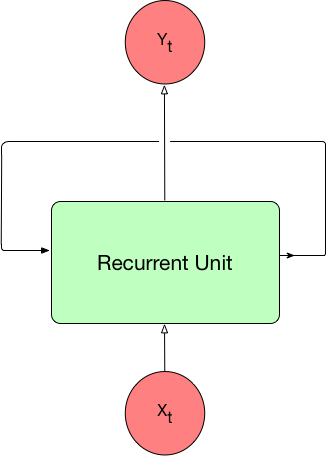
\includegraphics[width=2.0in]{Figures/recurrent1}
	\caption[Box figure]{Illustration of recurrent network}
\end{figure}

However, training conventional RNNs using back-propagation technique is difficult due to the vanishing gradient and exploding gradient problems\cite{bengio1994learning}. The gradient shifting problem make
also make it difficult for the network to remember long time dependency that longer than 5-10 time steps between input and output.
\section{Long Short term memory}
In order to address the problem above, a special recurrent network architecture Long-Short-Term Memory(LSTM) have been proposed\cite{hochreiter1997long}. LSTM and it's variations have been successfully applied to sequence prediction, translation and sequence labeling tasks. In the rest of this chapter I will introduce how LSTM and one of its variantion GRU(gated recurrent unit) works.\par
\subsection{Long short term memory}
To make it easier to understand the idea of LSTM, let unroll the loop in the network and then we got a fix length static version of the same network(figure 2.2). The operation in the two RNN version are the same, the difference is the static version only take fix length input and don't have to consider when to stop the iteration thus it runs faster.\par
\begin{figure}[h] 
	\centering
	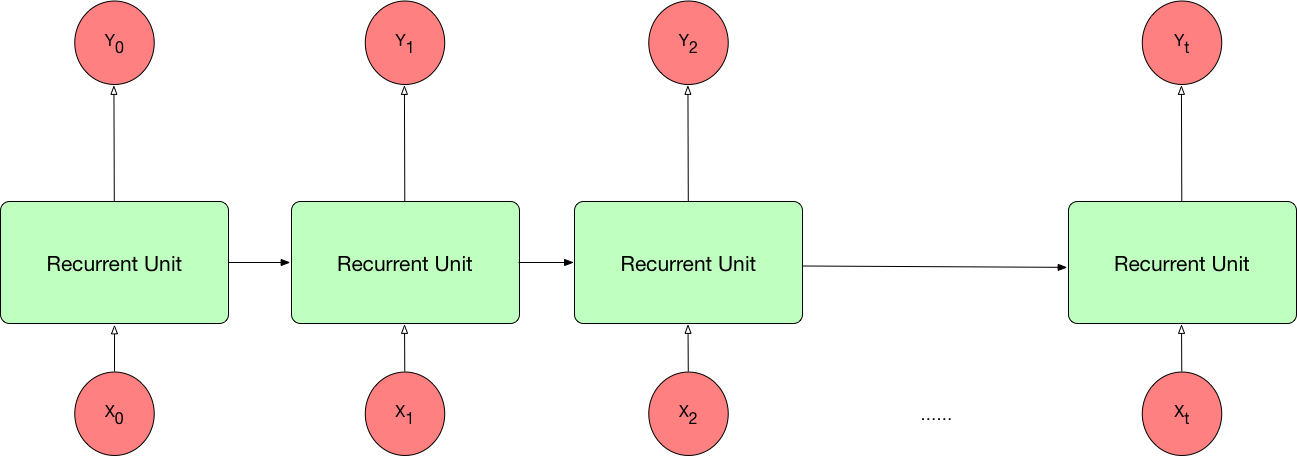
\includegraphics[width=6.0in]{Figures/recurrent2}
	\caption[Box figure]{Illustration of recurrent network}
\end{figure}

When we look at the inside of each recurrent unit(Cell), a conventional RNN can be represent as figure 2.3. The cell take the concatenation of input of time t and output of time t-1 as input. Going through a dense layer the cell will output the activation of the dense layer.\par  

LSTM also have the same loop structure of conventional RNN, but it has different structure inside the cell. Instead of having only a single dense layer in the cell, the LSTM cell has four dense layers. One of them is the counter-part in conventional RNN cell, the rest three, however, works as three "gates" controlling the behavior of the cell(figure 2.4).\par 

\begin{figure}[h] 
	\centering
	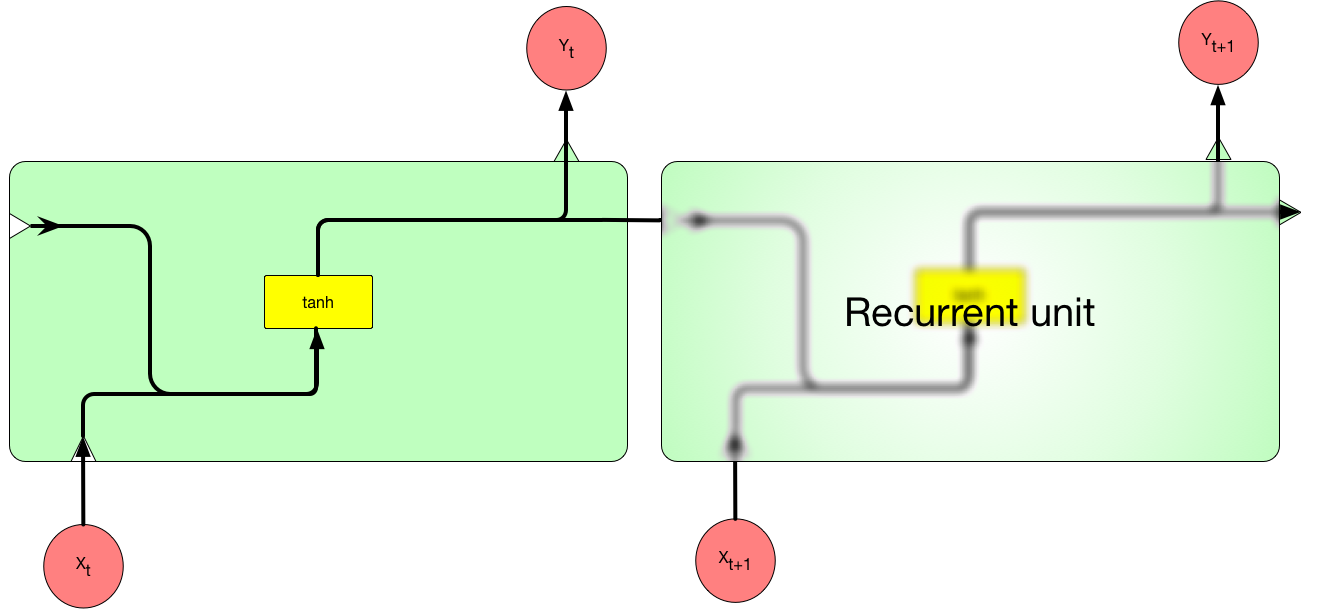
\includegraphics[width=6.0in]{Figures/recurrent3}
	\caption[Box figure]{Illustration of recurrent network}
\end{figure}

\begin{figure}[h] 
	\centering
	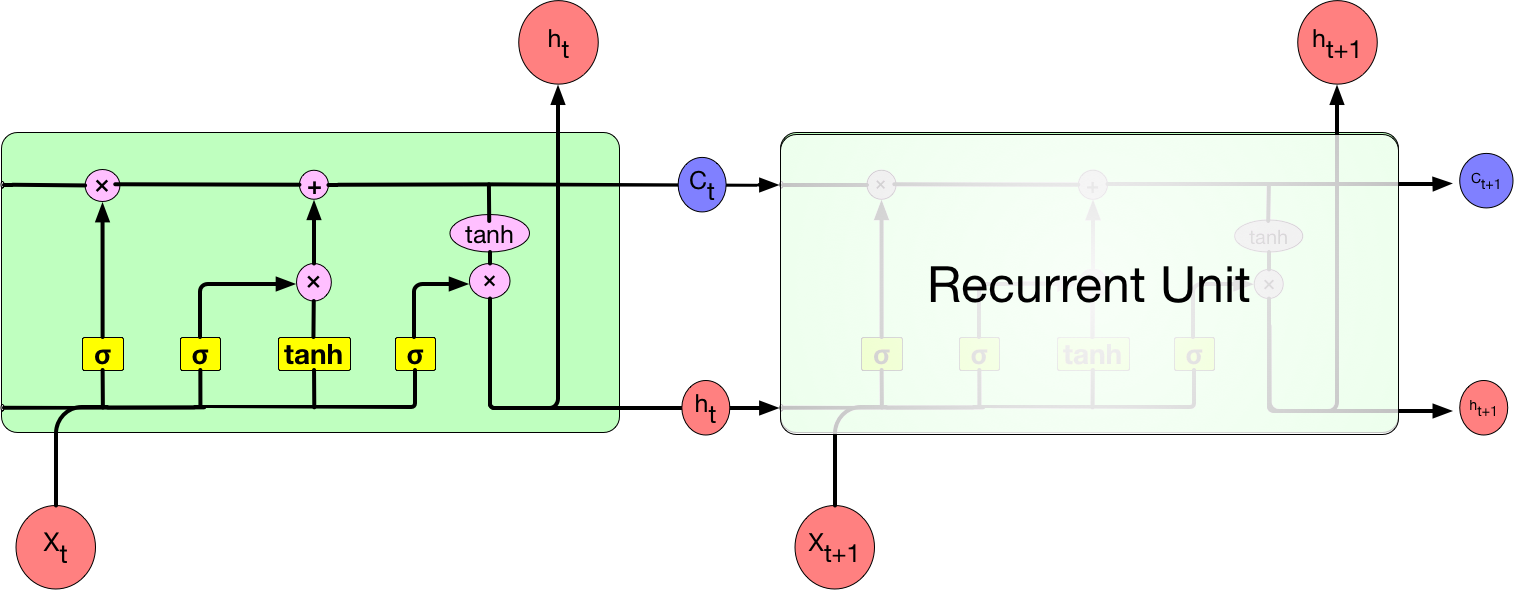
\includegraphics[width=6.0in]{Figures/recurrent4}
	\caption[Box figure]{Illustration of recurrent network}
\end{figure}

The first step of calculating the output $h_t$ of each time step is updating the cell state $C_t$. Because the output of each time step, is essentially the cell state masked by a weight matrix. In order to update the cell state, we need the output of the first three dense layer inside the cell which are forget gate layer, input gate layer and $tanh$ layer. The activation of these three layers can be calculated by using \ref{eq:0}, \ref{eq:1} and \ref{eq:2}. Then according to  \ref{eq:3} the network will decide how to update the cell state by forgetting some of the old state and remember some of the new input state.\par
After updated the cell state, the network will calculate the output of this time step using \ref{eg:4} and \ref{eg:5}
\begin{subequations} 
    \begin{align}
    	f_{ t }&=\sigma (W_{ f }\cdot [h_{t-1} , x_t] +b_f) \label{eq:0}\\	
        i_t &= \sigma(W_i \cdot[h_{t-1}, x_t] + b_i)\label{eq:1}\\
        \tilde {  {C _t } } &= tanh(W_c\cdot [h_{t-1}, x_t]+ b_c) \label{eq:2}
    \end{align}	
\end{subequations}




\begin{equation} \label{eq:3}
    C_t = f_t\ast C_{t-1} +i_t\ast \tilde{C}
\end{equation}

\begin{subequations}
    \begin{align}
        o_t = \sigma(W_o\cdot [h_{t-1}, x_t] +b_o) \label{eg:4}\\
        h_t = o_t \ast tanh(C_t) \label{eg:5}
    \end{align}
\end{subequations}

\par
\subsection{Gated recurrent unit}
\par
Here is how to display some in-line math, $x=\cos\theta$. Here is a numbered equation:
